
%(BEGIN_QUESTION)
% Copyright 2010, Tony R. Kuphaldt, released under the Creative Commons Attribution License (v 1.0)
% This means you may do almost anything with this work of mine, so long as you give me proper credit

Determine the approximate value of the {\it derivative} ($dy \over dx$) for this function where $x=-8$:

$$\includegraphics[width=15.5cm]{i04369x01.eps}$$

Choose the closest answer:

\begin{itemize}
\item{} $dy \over dx$ = +1
\vskip 10pt 
\item{} $dy \over dx$ = $-1$
\vskip 10pt 
\item{} $dy \over dx$ = +2
\vskip 10pt 
\item{} $dy \over dx$ = $-2$
\vskip 10pt 
\item{} $dy \over dx$ = +5
\vskip 10pt 
\item{} $dy \over dx$ = $-5$
\vskip 10pt 
\item{} $dy \over dx$ = 0
\end{itemize}

\vskip 20pt \vbox{\hrule \hbox{\strut \vrule{} {\bf Suggestions for Socratic discussion} \vrule} \hrule}

\begin{itemize}
\item{} What is most important when solving problems such as this is to be able to explain {\it why} (not just {\it how}) to arrive at the correct value.  Try explaining the process of differentiation in your own words, as it applies to this particular problem.
\item{} Sometimes the slope of a curved function at any given point is graphically shown by something called a {\it tangent line}.  Research what a ``tangent line'' is, and then draw a tangent line on this function at the point where $x = -8$.
\end{itemize}

\underbar{file i04369}
%(END_QUESTION)





%(BEGIN_ANSWER)

$dy \over dx$ = +2

%(END_ANSWER)





%(BEGIN_NOTES)


\vfil \eject

\noindent
{\bf Summary Quiz:}

Determine the approximate value of the {\it derivative} ($dy \over dx$) for this function where $x=-10$:

$$\includegraphics[width=15.5cm]{i04369x02.eps}$$

Choose the closest answer:

\vskip 10pt

0 \hskip 40pt +1 \hskip 40pt -1  \hskip 40pt +0.25  \hskip 40pt -0.25  \hskip 40pt +3 \hskip 40pt -3   


\vfil \eject


\noindent
{\bf Summary Quiz:}

Determine the approximate value of the {\it derivative} ($dy \over dx$) for this function where $x=4$:

$$\includegraphics[width=15.5cm]{i04369x02.eps}$$

Choose the closest answer:

\vskip 10pt

0 \hskip 40pt +1 \hskip 40pt -1  \hskip 40pt +0.25  \hskip 40pt -0.25  \hskip 40pt +3 \hskip 40pt -3   


\vfil \eject


\noindent
{\bf Summary Quiz:}

Determine the approximate value of the {\it derivative} ($dy \over dx$) for this function where $x=-4$:

$$\includegraphics[width=15.5cm]{i04369x02.eps}$$

Choose the closest answer:

\vskip 10pt

0 \hskip 40pt +1 \hskip 40pt -1  \hskip 40pt +0.25  \hskip 40pt -0.25  \hskip 40pt +3 \hskip 40pt -3   

\vfil \eject



\noindent
{\bf Summary Quiz:}

Determine the approximate value of the {\it derivative} ($dy \over dx$) for this function where $x=7$:

$$\includegraphics[width=15.5cm]{i04369x02.eps}$$

Choose the closest answer:

\vskip 10pt

0 \hskip 40pt +1 \hskip 40pt -1  \hskip 40pt +0.25  \hskip 40pt -0.25  \hskip 40pt +3 \hskip 40pt -3   



%INDEX% Mathematics, calculus: derivative (approximating derivative values at points on graph)

%(END_NOTES)


